\documentclass [a4paper,10pt]{article}
\newcommand{\n}[1]{\textbf{#1}}
\newcommand{\e}[1]{\textcolor{red}{#1}}
\linespread {1.5}
\usepackage[brazilian]{babel}
\usepackage[utf8]{inputenc}
\usepackage[T1]{fontenc}
\usepackage{amsfonts}
\usepackage{amsmath}
\usepackage{amssymb}
\usepackage{amsthm}
    \newtheorem{de}{Definicao}
    \newtheorem{te}{Teorema}
    \newtheorem{pa}{Prova}
    \newtheorem{cl}{Corolário}
    \newtheorem{pr}{Proposição}
\usepackage[ruled,vlined]{algorithm2e}
\usepackage{caption}
\usepackage{subcaption}
\usepackage{booktabs}
\usepackage{multirow}
\usepackage{fancyhdr}
\usepackage{verbatim}
\usepackage{alltt}
\usepackage{fancyvrb}
\usepackage{graphicx,xcolor}
\usepackage{listings}
\lstset{numbers=left,
stepnumber=1,
firstnumber=1,
numberstyle=\tiny,
extendedchars=false,
breaklines=flase,
tabsize=2,
showtabs=true,
tab=\textcolor{gray}{$\cdots$},
keywordstyle=\color{blue},
frame=tb,
basicstyle=\footnotesize,
stringstyle=\ttfamily,
showstringspaces=false}
\renewcommand{\lstlistingname}{Programa}
\renewcommand{\lstlistlistingname}{Lista de Listagens}
\usepackage[pdftex]{hyperref}
\hypersetup{colorlinks,%
linkcolor=red}

\begin{document}

\noindent\rule{\textwidth}{2pt}\\[-3mm]
    \linespread {0.7} {
    \begin{Verbatim}[fontsize=\small]
__/\\\\\\\\\\\\\\\__/\\\\\\\\\\\\\_________________/\\\\\\\\\\__        
 _\/\\\///////////__\/\\\/////////\\\_____________/\\\///////\\\_       
  _\/\\\_____________\/\\\_______\/\\\____________\///______/\\\__      
   _\/\\\\\\\\\\\_____\/\\\\\\\\\\\\\/____________________/\\\//___     
    _\/\\\///////______\/\\\/////////_____________________\////\\\__    
     _\/\\\_____________\/\\\_________________________________\//\\\_   
      _\/\\\_____________\/\\\________________________/\\\______/\\\__  
       _\/\\\\\\\\\\\\\\\_\/\\\_______________________\///\\\\\\\\\/___ 
        _\///////////////__\///__________________________\/////////_____
    \end{Verbatim}
    \begin{alltt}
        \hspace{1cm} Métodos Numéricos em ALgebra Linear (MAC0300)
    \end{alltt}
    \vspace{-3mm}
    \rule{\textwidth}{2pt}\\[-6mm]

    \begin{center}
        \n{Por}\\[-0.5mm]
        $\quad${\small Caio Vinícius Dadauto$\quad$7994808}\\[-2mm]
        {\tiny \n{22/11/2014}}\\[4mm]
    \end{center}

    \vspace{2.8cm}

    As implementações deste trabalho foram executadas em uma máquina com as seguites configurações:\\
    {\linespread{1}
        \begin{tabular}{l r}    
            \hspace{2.5cm}\n{\small OS}      & \small Arch Linux\\
            \hspace{2.5cm}\n{\small Kernel}  & \small x86\_64 Linux 4.1.5-1-ARCH\\
            \hspace{2.5cm}\n{\small CPU}     & \small Intel Core i5-4200 CPU @ 2.6GHz\\
            \hspace{2.5cm}\n{\small RAM}     & \small 3862MiB
        \end{tabular}
    }

    \section{Implementação}
    A implementação para o problema de quadrados mínimos utilizando refletores foi feita basicamente seguindo
    a rigor os passos sugeridos pelo livro \cite{livro1}. Grande parte das explicações concernentes a implementação estão
    indicadas em forma de comentario no proprio código. Para facilitar a compreensão da implementação, ao declarar as funções
    utilizadas durante o código foi indicado a qual parte do problema cada conjunto de função está relacionado. Os comentários
    se encontram sempre ao início de cada função e explica alguns detalhes da implementação e os objetivos de cada uma edstas
    funções.

    Para poder testar o programa, foi feita duas abordagens do problema de quadrados mínimos. A primeira é uma aborgem mais
    prática que consiste na seguinte situação, um certo usuário toma um conjunto de dados contendo pontos $(a, b)$ e a este conjunto
    quer ajustar um polinômio de grau $m - 1$. Dessa forma o usuário fornece um arquivo texto contendo o tamanho do conjunto,
    o grau do polinômio e o conjunto de pontos $(a, b)$. A partir deste arquivo texto o programa gera o sistema $Ax = b$, tomando
    cuidado na escolher da base de polinômios para gerar $A$ bem condicionada.
    Esta escolha foi feita baseada em \cite{livro2}, o que é basicamente
    determinar os valores máximo e mínimo entre os valores de $a$ e tomar a base como sendo potências da seguinte variável:
    \begin{equation}\label{base}
        s = \frac{a - \left(\frac{\mathrm{max} + \mathrm{min}}{2}\right)}{\mathrm{max} - \left(\frac{\mathrm{max} + \mathrm{min}}{2}\right)}
    \end{equation}


    A segunda aborgem está relacionada exclusivamente com os teste do programa. Esta abordagem consistem em fornecer ao programa
    um arquivo texto contendo explicitamente $A$ e $b$ do sistema $Ax = b$. A ídeia é fornecer $A$ com posto defeituoso para constatar
    se o programa de fato encontra tal problema. Neste caso de posto defeituoso, o porblema de quadrados mínimos assume infinitas
    soluções. Assim, ao resolver o MMQ, optou-se por tomar $y_2$ como vetor nulo em \cite{livro1}:
    \[
        R_{11}y_1 = c - R_{12}y_2
    \]
    esta escolha foi feita unicamente para fins práticos.

    Ao término do programa é impresso na tela o posto de $A$ e a solução $x$ do porblema de quadrados mínimos. Caso o usuário
    optou por inserir o conjunto de pontos ao invés de $A$ e $b$, o progrma imprime o polinômio que se ajusta aos pontos fornecidos.
    A impressão da solução $x$ é feita somente se $x$ possuir um tamanho ''legível", no caso com tamanho maior ou igual a 20.

    \section{Exemplos}
    \subsection{Constatação de Ajuste}
    Suponha que o usuário meça um conjunto de pontos e a este quer ajustar um polinômio de grau 2. Para exemplificar
    tal situação, tomemos o conjunto de pontos especificado no arquivo \texttt{exemplo1} como entrada do progrma.
    Assim, após resolver o problema de quadrados mínimos, obteve-se o seguinte ajuste ao conjunto de pontos:
    \begin{figure}[!ht]
        \centering
        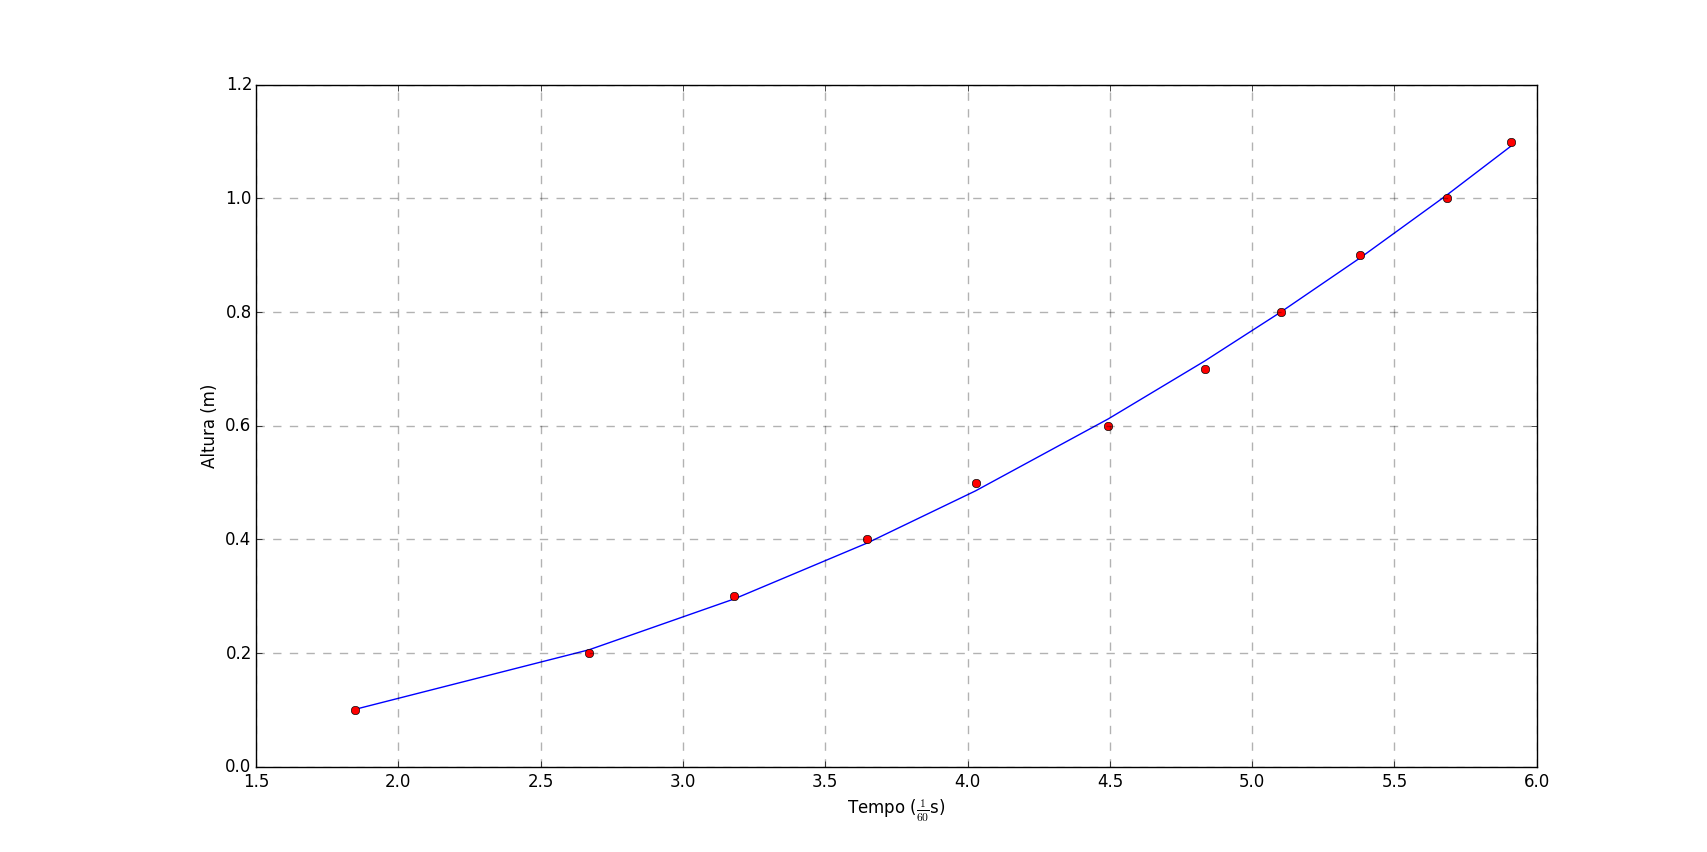
\includegraphics[scale=0.31]{exemplo1.png}
        \caption{Ajuste obtido para o conjunto de dados fornecido pelo arquivo \texttt{exemplo1}.}
    \end{figure}
    
    \subsection{Estimativa da Gravidade}
    Suponha um experimento em que o usuário quer determinar a gravidade local. Para isso ele decide abandonar um
    objeto com boa aerodinâmica a uma determinada autura do solo. Durante a queda ele anota a posição (em cm) com relação ao
    solo a cada $\frac{1}{60}s$, obtendo dessa forma um conjunto de pontos de posição contra o tempo.
    Assim, quer ajustar a estes dados a seguinte
    função:
    \begin{equation}\label{fisica}
        x = x_0 + v_0 t + \frac{1}{2}gt^2
    \end{equation}
    e com o valor de ajuste determinar $g$. Como está função nada mais é que um polinômio de segundo grau, basta fornecer
    ao porgrama um arquivo (\texttt(exemplo2)) contendo esse conjunto de dados.  
    
    O coeficiente obtido para $s^2$ foi de $32.4073$, a partir disso é possível determinar o coeficiente de $t^2$ através
    da expressão \eqref{base}. Coeficiente, este, que vale $0.1349$. Sabendo que a posição foi medida em centímetros, os
    instântes de tempo são da ordem de $\frac{1}{60}$s e, ainda, notando a constante $\frac{1}{2}$ na expressão \eqref{fisica},
    temos que:
    \[
        0.1349 = \frac{1}{72}g
    \]
    o que resulta em $g = 9.7128$, resultado que, por sua vez, é acurado. O ajuste obtido é apresentado na figura
    logo abaixo.
     
    \begin{figure}[!ht]
        \centering
        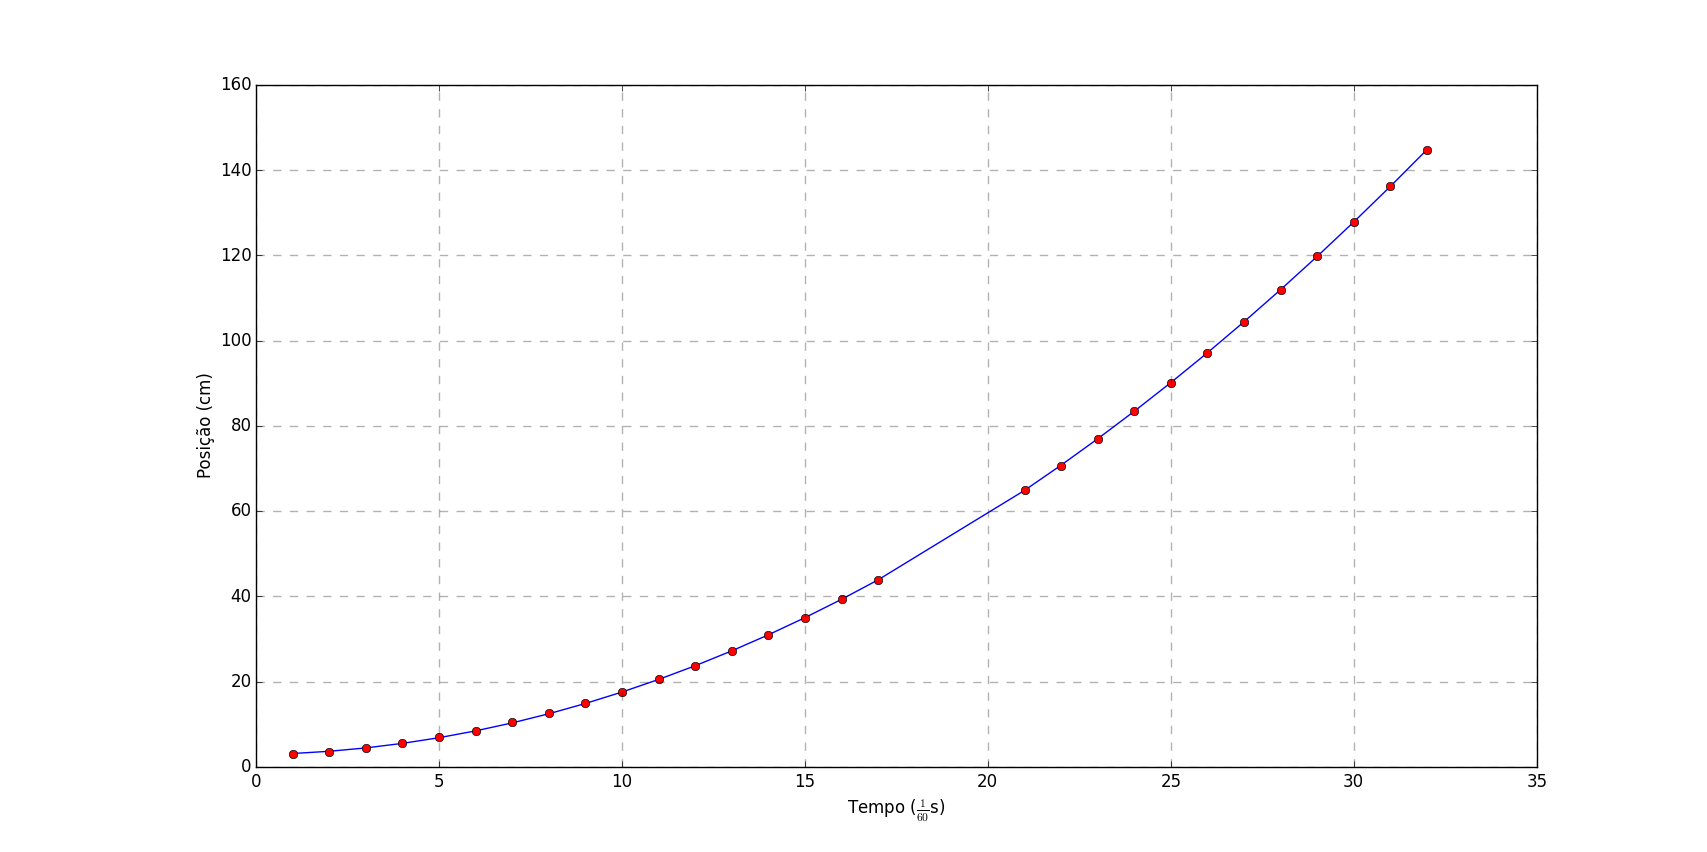
\includegraphics[scale=0.31]{exemplo2.png}
        \caption{Ajuste obtido para o conjunto de dados fornecido pelo arquivo \texttt{exemplo1}.}
    \end{figure}


    \subsection{Posto Incompleto}
    Para gerar $A$ com posto incompleto, utilizou-se o progrma do \texttt{ep1} que gera $A$ e $b$ aleatóriamente com $A$
    singular, ou seja, com posto imcompleto. A partir deste gerador, criou-se uma matriz $A$ quadrada de 700 linhas e
    singular, com posto 699. Esta $A$ e $b$ de $Ax = b$ estão salvos no arquivo \texttt{teste}. Tomando este arquivo como
    entrada do programa, constata-se que de fato o programa encontra o posto incompleto de $A$.

  \begin{thebibliography}{99}
      \bibitem{livro1} \emph{David S. Watkins,} Fundamentals of Matrix Compputation, Wiley, Third Edition.
      \bibitem{livro2} \emph{Math Works,} \texttt{http://www.mathworks.com/moler/leastsquares.pdf}
  \end{thebibliography}
    
\end{document}
    
